\documentclass[a4paper,11pt]{article}

\usepackage[margin=2.5cm]{geometry}
\usepackage{fontspec}
\setmainfont{TeX Gyre Pagella}
\usepackage{unicode-math}
\setmathfont{TeX Gyre Pagella Math}

\usepackage{tikz}
\usetikzlibrary{arrows.meta,shapes.geometric}
\usepackage{microtype}
\usepackage{enumitem}

\pagestyle{empty}
\setlength{\parindent}{0pt}
\setlength{\parskip}{0.4em}

\tikzset{
  node-d/.style={draw,fill=black,regular polygon,regular polygon sides=6,minimum size=5mm,inner sep=0pt,text=white,font=\tiny\bfseries},
  node-a/.style={draw,fill=black!70,regular polygon,regular polygon sides=3,minimum size=5mm,inner sep=0pt,text=white,font=\tiny\bfseries},
  node-t/.style={draw,circle,minimum size=5mm,inner sep=0pt,line width=0.4pt,font=\tiny},
  node-o/.style={draw,fill=black!15,rectangle,minimum size=5mm,inner sep=0pt,font=\tiny},
  node-i/.style={draw,diamond,minimum size=6mm,inner sep=0pt,line width=0.4pt,font=\tiny},
}

\begin{document}

%============================================================
%  SIDE 1 — FORSIDE
%============================================================
\vspace*{4cm}

\begin{center}
{\Huge\scshape Atlas over Formlære}\\[0.8em]
{\large\itshape Ei grafisk grammatikk over traktaten}
\end{center}

\vspace{3cm}

\begin{center}
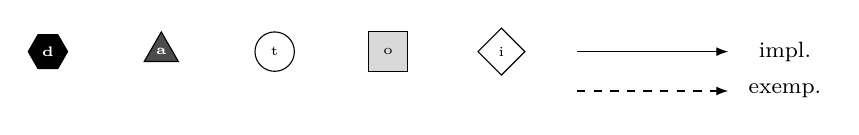
\begin{tikzpicture}[x=1.2cm,y=1cm]
  \node[node-d] at (0, 0)  {d};
  \node[node-a] at (1.2, 0){a};
  \node[node-t] at (2.4, 0){t};
  \node[node-o] at (3.6, 0){o};
  \node[node-i] at (4.8, 0){i};

  \draw[-{Latex[length=1.5mm]},line width=0.4pt] (5.6, 0) -- (7.2, 0);
  \draw[-{Latex[length=1.5mm]},line width=0.4pt,dashed] (5.6, -0.5) -- (7.2, -0.5);

  \node[font=\footnotesize] at (7.8, 0) {impl.};
  \node[font=\footnotesize] at (7.8, -0.5) {exemp.};
\end{tikzpicture}
\end{center}

\vspace{3cm}

\begin{center}
{\large Iver Raknes Finne}\\[0.3em]
{\itshape iver.raknes.finne@stud.aho.no}\\[0.6em]
Arkitektur- og designhøgskolen i Oslo  \  2026
\end{center}

\newpage

%============================================================
%  SIDE 2 — INNHALD OG LESINGSRETTLEIING
%============================================================
\vspace*{0.5cm}

\begin{center}
{\Large\scshape Innhald og lesingsrettleiing}
\end{center}

\vspace{0.5em}

\hrule

\vspace{0.5em}

Atlaset er ei grafisk grammatikk over FORMLÆRE som avslører den logiske arkitekturen i traktaten. Same alfabetet vart brukt i alle diagramma, og ein enkelt lesingsregel held for alle: \emph{teikna viser dei næraste logiske avhengigheitene mellom proposisjonar, ikkje dei transitive}.

\vspace{0.5em}

\hrule

\vspace{0.5em}

{\scshape Dokumentrekkja}

\begin{enumerate}[leftmargin=*,itemsep=0.15em]
\item \textbf{Notasjon}  alfabetet og komponentkartet. To sider i A4-stående format. Set opp grammatikken for alle diagramma som følgjer.
\item \textbf{Proposisjonsgraf, seksjon 1}  \emph{formverda er alt som er tilfelle}. Fem epistemiske band frå vera til viten.
\item \textbf{Proposisjonsgraf, seksjon 2}  \emph{ikkje alle posisjonar er like sannsynlege}. Fyrste postulat og fyrste empiri. Konfluens ved 2.21.
\item \textbf{Proposisjonsgraf, seksjon 3}  \emph{seleksjonstrykka spenner ut eit landskap}. Rein karakterisering. Ingen postulat.
\item \textbf{Proposisjonsgraf, seksjon 4}  \emph{landskapet er dynamisk}. Eitt postulat, tredobbel fan-out, observasjonstung.
\item \textbf{Proposisjonsgraf, seksjon 5}  \emph{verda rommar agentar}. Trippelteforeldreskap ved 5.7. Atlaset sitt høgdepunkt.
\item \textbf{Proposisjonsgraf, seksjon 6}  \emph{forma oppstår mellom agentane}. Konfluens ved 6.14. Formgjevar-designar-skiljet.
\item \textbf{Proposisjonsgraf, seksjon 7}  \emph{forma viser kor langt omhugen rakk}. Tre postulat på rad. Den etiske kjernen.
\item \textbf{Proposisjonsgraf, seksjon 8}  \emph{forma er ei sannsynsfordeling}. Matematisk lukking. Åtte nodar.
\item \textbf{Tilleggsdiagram: skalahierarki}  dei sytten nivåa av kognitiv lyskjegle, visualisert som stabla lyskjegler med proporsjonal storleik.
\end{enumerate}

\vspace{1em}

\hrule

\vspace{1em}

{\scshape Tolkingsnøkkel for sjanger}

Ved å sjå atlaset samla, står fire sjangrar fram i traktaten:

\begin{itemize}[leftmargin=*,itemsep=0.2em]
\item \emph{Oppfinningsseksjonar} (1, 2, 5, 6) innfører ny ontologi og har konfluens.
\item \emph{Karakteriseringsseksjonar} (3) karakteriserer eksisterande ontologi utan risiko.
\item \emph{Dynamisk karakterisering} (4) har eitt postulat med parallelle konsekvenskjeder.
\item \emph{Normativ karakterisering} (7) har fleire postulat som ber den etiske argumentasjonen.
\end{itemize}

Seksjon 8 står i særstilling som rein matematisk lukking.

\vspace{0.6em}

\hrule

\vspace{0.6em}

Atlaset kan lesast på tre måtar. Byrj med notasjonen for å læra alfabetet; les deretter seksjon 1 til 8 lineært for å følgje traktaten si eiga rørsle; eller hopp til den seksjonen som er mest relevant for det aktuelle spørsmålet. Kvar graf er sjølvforklarande gjennom tekstpanela under.

\end{document}
